\documentclass[10pt]{article}

\usepackage{amsmath}

\newcommand{\myvec}[1]{\ensuremath{\begin{pmatrix}#1\end{pmatrix}}}

\newcommand{\mydet}[1]{\ensuremath{\begin{vmatrix}#1\end{vmatrix}}}

\newcommand{\solution}{\noindent \textbf{Solution: }}

\providecommand{\brak}[1]{\ensuremath{\left(#1\right)}}

\providecommand{\norm}[1]{\left\lVert#1\right\rVert}
\usepackage{graphicx}
\usepackage{float}
\let\vec\mathbf
\title{Coordinate Geometry}
\author{karthik(karthik.pyla@sriprakashschools.com)}

\begin{document}
\maketitle
\section*{Class 10$^{th}$ Maths - Chapter 7}
This is Problem-5 from Exercise 7.3
\begin{enumerate}
\item  QUESTION: Median of a triangle divides it into two equal triangles of same areas.Verify this result for triangle ABC whose vertices are A(4,-6) B(3,-2) C(5,2)
\end{enumerate}
\solution \\
\begin{align}
\vec{A} &= \myvec{4\\-6}\\
\vec{B} &= \myvec{3\\-2} \\
\vec{C} &= \myvec{5\\2}\\ 
\end{align}
Let the $\vec{AP}$ be the median from $\vec{A}$ to side $\vec{BC}$. Hence, 
\begin{align}
    \vec{P} &= \frac{(1)\vec{C}+(1)\vec{B}}{1+1}\\
    \vec{P} &= \frac{(1)\myvec{5\\2}+(1)\myvec{3\\-2}}{2}\\
    \vec{P} &= \myvec{4\\0}\\   
\end{align}
\begin{align}
\\Area of triangle ABP&=\frac{1}{2}\norm{ \myvec {\vec{BP}\times \vec{BA}}}\\&=\frac{1}{2}\mydet{ {1}&{1} \\{2}&{-4}}\\ &=\frac{1}{2}\norm{-4-(2)}\\&=\frac{1}{2}(-6)\\&=-3 sq.units
\end{align}
However the area cannot be negative . Therefore the area of triangle ABP is equal to 3 square units
\begin{align}
\\Area of triangle ACP&=\frac{1}{2}\mydet{ \myvec {\vec{CP}\times \vec{CA}}}\\&=\frac{1}{2}\mydet{ {-1}&{-1} \\{-2}&{-8}}\\ &=\frac{1}{2}\norm{8-2}\\&=\frac{1}{2}(6)\\&=3 sq.units
\end{align}

The area of both sides is the same. Thus, median AD has divided ABC into two triangles of equal areas.
\begin{figure}[H]
			\centering
			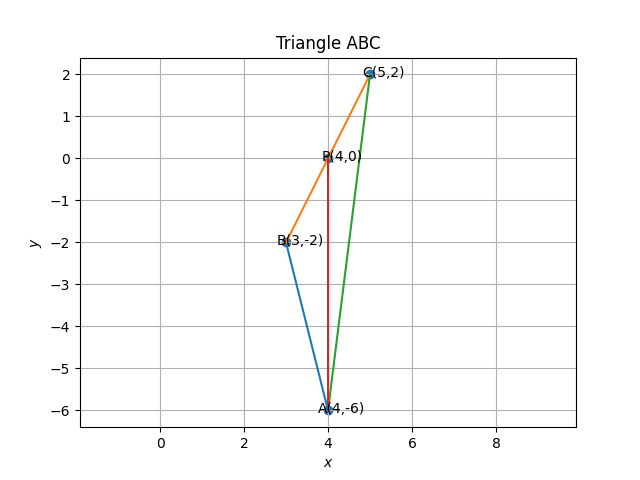
\includegraphics[width=\columnwidth]{figs/Figure_1.png}
			\caption{Triangle ABC}
			\label{fig:tri1}
		\end{figure}

\end{document}
